\documentclass{math}

\usepackage{circuitikz}
\usepackage{tikz}

\title{University Physics 2}
\author{Alvin Lin}
\date{January 2018 - May 2018}

\begin{document}

\maketitle

\section*{Circuits}
We will start with a microscopic pictures of current and resistance.
\begin{center}
  \begin{circuitikz}
    \draw (0,0) to[battery, label=\( \Delta V \)] (0,2) -- (4,2)
      to[resistor, label=R] (4,0) -- (0,0);
   \draw[->] (1.5,2.5) -- (2.5,2.5) node[pos=0.5,above] {\( I \)};
  \end{circuitikz}
\end{center}
Current will flow clockwise in this example, from the positive terminal of the
battery through the wires, into the negative terminal. If we look at a small
section of wire at the top.
\begin{center}
  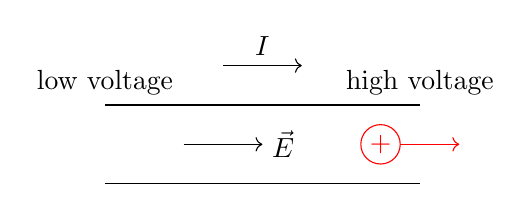
\begin{tikzpicture}
    \draw (0,0) -- (4,0);
    \draw (0,1) node[above] {low voltage} -- (4,1) node[above] {high voltage};
    \draw[->] (1.5,1.5) -- (2.5,1.5) node[pos=0.5,above] {\( I \)};
    \draw[->] (1,0.5) -- (2,0.5) node[right] {\( \vec{E} \)};
    \draw[red] (3.5,0.5) circle (0.25) node[] {+};
    \draw[red,->] (3.75,0.5) -- (4.5,0.5);
  \end{tikzpicture}
\end{center}
We define current, \( I \) as the charge moved through the wire, per unit time.
\[ I = \ddiff{Q}{t} = nqAV_d \]
Sometimes, we will want the current density:
\[ J = \frac{I}{A} = nqV_d \]
All the constants can be defined and rewritten:
\[ \rho = \frac{E}{J} \]
where \( \rho \) is the resistivity of the wire. It is a fundamental property of
a material independent of area or density.
\[ [\rho] = \frac{[E]}{[J]} = \frac{\frac{V}{m}}{\frac{A}{m^2}} =
  \frac{V\cdot m}{A} \]
\begin{align*}
  E &= \rho J \\
  EL &= \rho JL \\
  \Delta V &= \frac{\rho IL}{A} \\
  &= \frac{\rho L}{A}I \\
  R &= \frac{\rho L}{A} \\
  \Delta V &= IR
\end{align*}
This is known as Ohm's Law, where the units of resistance \( R \) are measured
in ohms (\( \Omega \)). All these derivations are done in terms of a positive
charge, but in a wire, the charges that are moving are electrons.
\begin{center}
  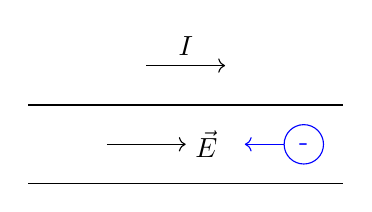
\begin{tikzpicture}
    \draw (0,0) -- (4,0);
    \draw (0,1) -- (4,1);
    \draw[->] (1.5,1.5) -- (2.5,1.5) node[pos=0.5,above] {\( I \)};
    \draw[->] (1,0.5) -- (2,0.5) node[right] {\( \vec{E} \)};
    \draw[blue] (3.5,0.5) circle (0.25) node[] {-};
    \draw[blue,->] (3.25,0.5) -- (2.75,0.5);
  \end{tikzpicture}
\end{center}

\subsection*{Temperature Dependence of Resistance}
Resistivity depends on temperature:
\[ (\rho-\rho_{\circ}) = \rho_{\circ}\alpha(T-T_{\circ}) \]
where \( \rho \) is resistivity, \( T \) is temperature, \( \alpha \) is the
temperature coefficient, and \( T_{\circ},\rho_{\circ} \) are reference values.
Note that this is similar to the equation of a line. Thus, the temperature
coefficient can be determined by measuring these values and determining the
slope of the line plotted by the resistivity at certain temperatures.

\subsection*{Power}
Power is energy per unit time. Recall that current is change in current over
unit time.
\[ I = \frac{\Delta Q}{\Delta t} \quad \Delta Q = I\Delta t \]
With potential energy:
\begin{align*}
  \Delta U &= \Delta QV \\
  \Delta U &= I\Delta tV \\
  \frac{\Delta U}{\Delta t} &= IV \\
  P &= IV
\end{align*}
In relation to Ohm's Law:
\[ P = IV = I^2R = \frac{V^2}{R} \]

\subsection*{Equivalent Resistance (In Series)}
\begin{center}
  \begin{circuitikz}
    \draw (0,0) to[battery, label=\( \Delta V \)] (0,2)
      to[resistor,label=\( R_1 \)] (2,2)
      to[resistor,label=\( R_2 \)] (4,2) -- (4,0) -- (0,0);
  \end{circuitikz} \\[1cm]
  \begin{circuitikz}
    \draw (0,0) to[battery, label=\( \Delta V \)] (0,2)
      to[resistor,label=\( R_{eq} \)] (4,2) -- (4,0) -- (0,0);
  \end{circuitikz}
\end{center}
From conservation of charge:
\[ I_1 = I_2 = I_{eq} \]
From conservation of energy and the equivalent circuit:
\[ \Delta V = \Delta V_1+\Delta V_2 \]
From the equivalent circuit:
\begin{align*}
  \Delta V &= IR_{eq} \\
  \Delta V_1+\Delta V_2 &= IR_{eq}
\end{align*}
Using Ohm's Law:
\begin{align*}
  IR_1+IR_2 &= IR_{eq} \\
  R_1+R_2 &= R_{eq}
\end{align*}
Compared to capacitance:
\[ \frac{1}{C_{eq}} = \frac{1}{C_1}+\frac{1}{C_2} \]

\subsection*{Equivalent Resistance (In Parallel)}
\begin{center}
  \begin{circuitikz}
    \draw (0,0) to[battery, label=\( \Delta V \)] (0,2) -- (2,2)
      to[resistor,label=\( R_1 \)] (2,0) -- (0,0);
    \draw (2,2) -- (4,2)
      to[resistor,label=\( R_2 \)] (4,0) -- (2,0);
  \end{circuitikz} \\[1cm]
  \begin{circuitikz}
    \draw (0,0) to[battery, label=\( \Delta V \)] (0,2) -- (2,2)
      to[resistor,label=\( R_{eq} \)] (2,0) -- (0,0);
  \end{circuitikz}
\end{center}
From conservation of energy:
\[ \Delta V = \Delta V_1 = \Delta V_2 \]
From conservation of charge:
\[ I = I_1+I_2 \]
Using Ohm's Law:
\begin{align*}
  \frac{\Delta V}{R_{eq}} &= \frac{\Delta V}{R_1}+\frac{\Delta V}{R_2} \\
  \frac{1}{R_{eq}} &= \frac{1}{R_1}+\frac{1}{R_2} \\
  R_{eq} &= \frac{R_1R_2}{R_1+R_2}
\end{align*}

\subsection*{Kirchhoff's Laws}
At a junction or node, the current going in is equal to the current going out.
\[ I_{in} = I_{out} \]
\begin{center}
  \begin{tikzpicture}
    \draw[->,thick] (-2,0) -- (0,0) node[pos=0.5,above] {\( I_1 \)};
    \draw[->,thick] (0,0) -- (2,0) node[pos=0.5,above] {\( I_2 \)};
    \draw[->,thick] (0,0) -- (0,-2) node[pos=0.5,right] {\( I_3 \)};
  \end{tikzpicture}
\end{center}
\[ I_1 = I_2+I_3 \]
This arises from the conservation of current/charge and is always true in a
steady state. For a loop in a circuit, conservation of energy says:
\begin{center}
  \begin{circuitikz}
    \draw (0,0) to[battery, label=\( \Delta V_{battery} \)] (0,2) -- (2,2)
      to[resistor,label=\( R \)] (2,0) -- (0,0);
  \end{circuitikz}
\end{center}
\begin{align*}
  \Delta V_{total} &= 0 \\
  \Delta V_{battery}+\Delta V_{resistor} &= 0 \\
  \Delta V_{battery} &= -\Delta V_{resistor} \\
  \Delta E &= 0 = \Delta U = q\Delta V
\end{align*}
The voltage drop is zero for a closed loop. The voltage drop across a resistor
is negative if the loop chosen is in the same direction as the current. The
voltage drop is positive if the opposite is true. For a battery, the voltage
drop across it is positive if the loop goes from negative to positive.

\subsubsection*{Solving Kirchhoff's Law Problems}
\begin{enumerate}
  \item Draw currents through each element. If you don't know the directions,
  guess.
  \item Identify the number of loops and nodes.
  \item Draw the chosen loops.
  \item Write down one equation for each node and loop using Kirchhoff's Law.
  \item Solve it as a system of equations.
\end{enumerate}

\subsubsection*{Example}
\begin{center}
  \begin{circuitikz}
    \draw (0,0) to[battery, label=1.5 V] (0,4)
      to[resistor, label=\mbox{\( R_{1} = 1000 \Omega \)}] (4,4)
      to[resistor, label=\mbox{\( R_{3} = 100 \Omega \)}] (4,0) -- (0,0);
    \draw (4,0) -- (8,0)
      to[battery, l_=1.5 V] (8,4)
      to[resistor, l_=\mbox{\( R_{2} = 220 \Omega \)}] (4,4);
  \end{circuitikz}
\end{center}
This yields a few equations. We will use these three to solve for the voltage
drop:
\begin{align*}
  1.5-\Delta V_1-\Delta V_3 &= 0 \\
  1.5-\Delta V_2-\Delta V_3 &= 0 \\
  I_1+I_2 &= I_3
\end{align*}
We can substitute with Ohm's Law to yield a system of equations to solve for the
voltage drops:
\begin{align*}
  1.5-\Delta V_1-\Delta V_3 &= 0 \\
  1.5-\Delta V_2-\Delta V_3 &= 0 \\
  \frac{\Delta V_1}{R_1}+\frac{\Delta V_2}{R_2} &= \frac{\Delta V_3}{R_3} \\
  \Delta V_1 &= \frac{55}{57} \\
  \Delta V_2 &= \frac{55}{57} \\
  \Delta V_3 &= \frac{61}{114}
\end{align*}

\subsection*{RC Circuits}
\begin{center}
  \begin{circuitikz}
    \draw (0,0) to[battery, label=\( \epsilon \)] (0,2)
      to[capacitor, label=C] (2,2)
      to[resistor, label=R] (2,0) -- (0,0);
  \end{circuitikz}
\end{center}
We can analyze this circuit using Kirchhoff's Law as well.
\begin{align*}
  \epsilon-\Delta V_C-\Delta V_R &= 0 \\
  \epsilon-\frac{Q}{C}-IR &= 0 \\
  I &= \ddiff{Q}{t} \\
  I &= \frac{\epsilon}{R}-\frac{Q}{RC} \\
  \ddiff{}{t}I &= \ddiff{}{t}\bigg[\frac{\epsilon}{R}-\frac{Q}{RC}\bigg] \\
  \ddiff{I}{t} &= 0-\frac{1}{RC}\ddiff{Q}{t} \\
  \ddiff{I}{t} &= -\frac{1}{RC}I \\
  I(t) &= I_{\circ}\e^{-\frac{1}{RC}t}
\end{align*}
This is the equation of the current through an RC circuit with an uncharged
capacitor with \( \tau = RC \) as the time constant. We can also calculate
the charge as it changes over time:
\begin{align*}
  I &= \ddiff{Q}{t} \\
  \ddiff{Q}{t} &= \frac{\epsilon}{R}\e^{\frac{-t}{RC}} \\
  Q(t) &= \int_{0}^{t}\frac{\epsilon}{R}\e^{\frac{-t'}{RC}}\diff{t'} \\
  &= -\frac{\epsilon}{R}RC\e^{-t}{RC}+K \\
  Q(0) = 0 \\
  K &= \epsilon C \\
  Q(t) &= \epsilon C(1-\e^{-t}{RC})
\end{align*}
When the capacitor is discharging:
\begin{align*}
  \delta V_C &= \delta V_R \\
  \frac{Q}{C} &= IR = -\ddiff{Q}{t}R \\
  \frac{\diff{Q}}{Q} &= -\frac{1}{RC}\diff{t} \\
  \int\frac{\diff{Q}}{Q} &= -\int\frac{1}{RC}\diff{t} \\
  \ln(\frac{Q}{Q_0}) &= \frac{-t}{RC} \\
  Q(t) &= Q_{\circ}\e^{\frac{-t}{RC}} \\
  I(t) &= \ddiff{Q}{t} = \frac{-Q_{\circ}}{RC}\e^{\frac{-t}{RC}}
\end{align*}

\begin{center}
  You can find all my notes at \url{http://omgimanerd.tech/notes}. If you have
  any questions, comments, or concerns, please contact me at
  alvin@omgimanerd.tech
\end{center}

\end{document}
